\section{Microsoft Excel Configuration}
\label{sec.tut.simsinter.excel}

\begin{enumerate}

\item The ``SinterConfigGUI'' can be launched from FOQUS, via the
  \textbf{\underline{Create/Edit}} button found in
  \textbf{\underline{File}}$\rightarrow$ \textbf{\underline{Add/Update Model to
      Turbine}}    or ``SinterConfigGUI'' may be  run on its
  own by selecting \textbf{\underline{CCSI Tools}} $\rightarrow$
  \textbf{\underline{FOQUS}} $\rightarrow$
  \textbf{\underline{SinterConfigGUI}} from the Start menu.

\item	The splash window displays, as shown in Figure \ref{fig.sinter.acm.splash}.  The user may click the splash screen to proceed, or wait 10 seconds for it to close automatically.
\begin{figure}[H]
	\begin{center}
		\includegraphics[scale=0.55]{Chapt_sinter/figs/ap/01_Splash_Screen}
		\caption{SinterConfigGUI Splash Screen}
		\label{fig.sinter.excel.splash}
	\end{center}
\end{figure}

\item	The SinterConfigGUI Open Simulation window displays (Figure \ref{fig.sinter.acm.openpage}). If ``SinterConfigGUI'' was
  opened from FOQUS, the filename text box already contains the
  correct file.  To proceed immediately click \textbf{\underline{Open File and
  Configure Variables}} or click \textbf{\underline{Browse}} to search for the
  file. For this tutorial, a fresh copy of the BMI test is opened.  It
  can be found at: 

C:\textbackslash SimSinterFiles\textbackslash
  Excel\_Install\_Test\textbackslash exceltest.xlsm.
  
	\begin{figure}[H]
		\begin{center}
			\includegraphics[scale=0.55]{Chapt_sinter/figs/ap/02_FileOpenScreen}
			\caption{SinterConfigGUI Open Simulation Screen}
			\label{fig.sinter.excel.openpage}
		\end{center}
	\end{figure}


\item Microsoft Excel starts in the background.  This is so the user can observe things about the worksheet while working on the configuration file.

\item	In the ``SinterConfigGUI'' the SinterConfigGUI Simulation Meta-Data page is now displayed (Figure \ref{fig.sinter.excel.savename}). The
  first and most important piece of metadata is \textbf{\underline{Save Location}} at
  the top of the window.  This is where the sinter configuration file is saved. 
  The system attempts to locate a reasonable file location and file name; however, the user must confirm the correct file location, since it automatically overwrites whatever filename currently exists.
\begin{figure}[H]
	\begin{center}
		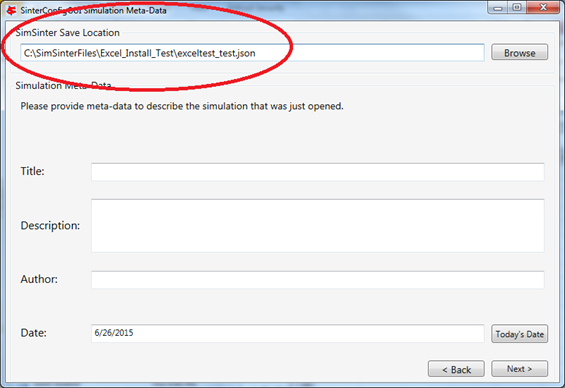
\includegraphics[scale=0.55]{Chapt_sinter/figs/Excel/04_MetaDataSave}
		\caption{SinterConfigGUI Simulation Meta-Data Save Text Box}
		\label{fig.sinter.excel.savename}
	\end{center}
\end{figure}

\item Continue to complete in the remaining fields and click \textbf{\underline{Next}}. 

\item In the SinterConfigGUI Variable
      Configuration Page, (Figure
  \ref{fig.sinter.excel.variableempty}) notice that the Excel setting
  variable \textbf{\underline{macro}} is already included in the
  \textbf{\underline{Selected Input Variables.}}  If the Excel spreadsheet has a macro that should be run after SimSinter sets the inputs, but before SimSinter gets the outputs, enter the macros name in the \textbf{\underline{Name}} text box.  If the default is left blank, no macro is run (unless a name is supplied in the input variables when running the simulation).
\begin{figure}[H]
	\begin{center}
		\includegraphics[scale=0.55]{Chapt_sinter/figs/Excel/06_VariablesEmpty}
		\caption{SinterConfigGUI Variable Configuration Page before Input}
		\label{fig.sinter.excel.variableempty}
	\end{center}
\end{figure}

\item The Excel simulation has the same \textbf{\underline{Variable
      Tree}} structure as Aspen Plus, as shown in (Figure
  \ref{fig.sinter.excel.variableselected}).  Only the variables in the
  active section of the Excel spreadsheet appear
  in the \textbf{\underline{Variable Tree}}.  If, for some reason, a cell does not appear
  the in tree, the user may manually enter the cell into the \textbf{\underline{Selected Path}} text box.  In this case, select the ``height\$C\$4'' variable.

Note: Row is first in the \textbf{\underline{Variable Tree}}, yet column is first in the \textbf{\underline{Path}}.

\begin{figure}[H]
	\begin{center}
		\includegraphics[scale=0.55]{Chapt_sinter/figs/Excel/07_VariablesSelected}
		\caption{SinterConfigGUI Variable Configuration Page Selecting a Variable from the Excel Variable Tree}
		\label{fig.sinter.excel.variableselected}
	\end{center}
\end{figure}

\item If the user double-clicks, presses enter, clicks \textbf{\underline{Preview}}, or clicks \textbf{\underline{Lookup}},
the  variable will be displayed in the \textbf{\underline{Preview Variable}} frame.  Click the \textbf{\underline{Make Input}} button to make the variable an input variable.  Now the variable is in the \textbf{\underline{Selected Input Variables}} section, and its meta-data may be edited (Figure \ref{fig.sinter.excel.variableinputs}).
\begin{figure}[H]
	\begin{center}
		\includegraphics[scale=0.55]{Chapt_sinter/figs/Excel/08_VariablesInput}
		\caption{SinterConfigGUI Variable Configuration Page Description ``Joe's Height''}
		\label{fig.sinter.excel.variableinputs}
	\end{center}
\end{figure}

\item Enter an output variable (such as, ``BMI\$C\$3''), by selecting the variables in the \textbf{\underline{Variable Tree}}, clicking \textbf{\underline{Preview}}, and then clicking \textbf{\underline{Make Output}} (Figure \ref{fig.sinter.excel.variableoutput}).

\begin{figure}[H]
	\begin{center}
		\includegraphics[scale=0.55]{Chapt_sinter/figs/Excel/09_VariablesOutput}
		\caption{SinterConfigGUI Variable Configuration Page Selecting Excel Output Variables}
		\label{fig.sinter.excel.variableoutput}
	\end{center}
\end{figure}

\item The simulation is now set up.  To save the configuration file, click \textbf{\underline{Finish}} or press CTRL+S.  The file is saved to the location that was set on the SinterConfigGUI Simulation Meta-Data window.  A user can save a copy under a different name, by navigating back to the SinterConfigGUI Simulation Meta-Data window using \textbf{\underline{Back}}, and then changing the name.  This creates a second version of the file.

\end{enumerate}

